% Trabajo Final de Grado
% Author: Eric Ríos Hamilton <alu0101549835@ull.edu.es>
% Chapter: GraphicsAndVisualAssets 
% ----------------------------------------------------
\chapter{Graphics and Visual Assets} \label{chap:GraphicsAndVisualAssets}
Due to the visual nature of the project, several graphical assets have been created and sourced to enhance presentation.

\section{Materials}
All materials used in this project, except for those packaged with imported 3D models, have been downloaded from FreePBR\footnote{\href{https://freepbr.com/}{FreePBR} - \url{https://freepbr.com/}}.
Some of those used to build terrain materials can be seen in Figure \ref{fig:pbr_mats}.

%% ===================================================
\begin{figure}[H]
    \centering
    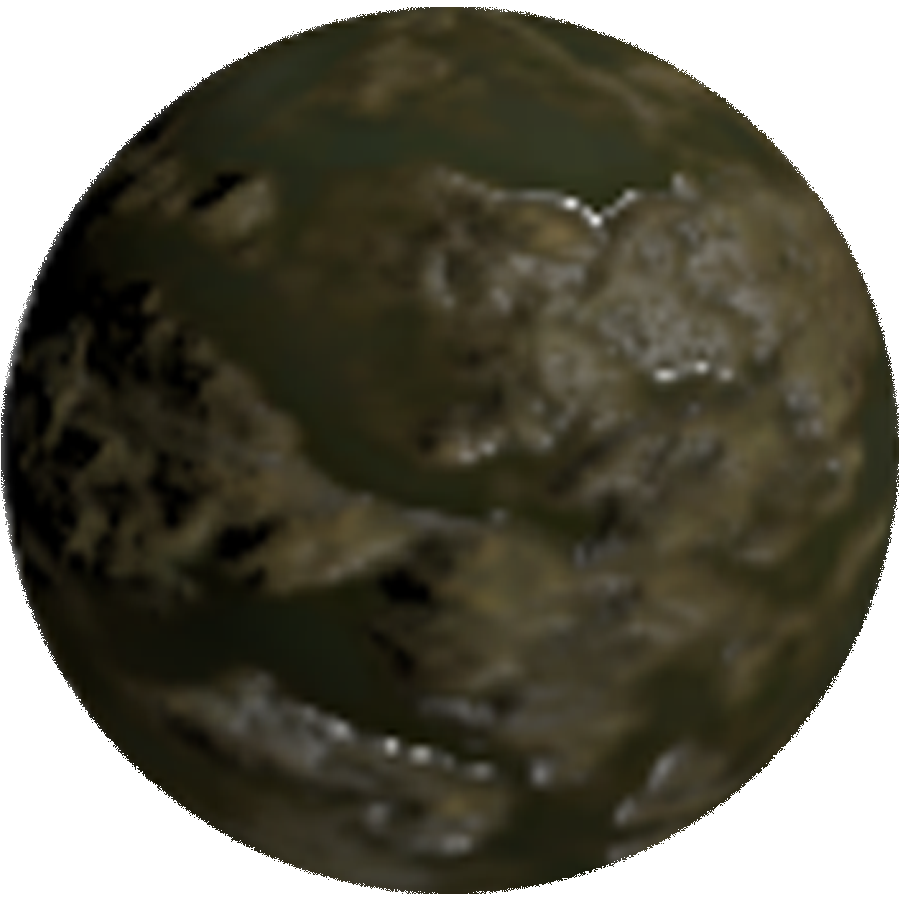
\includegraphics[width=0.24\textwidth]{Memoria/images/tidal_pool.png}
    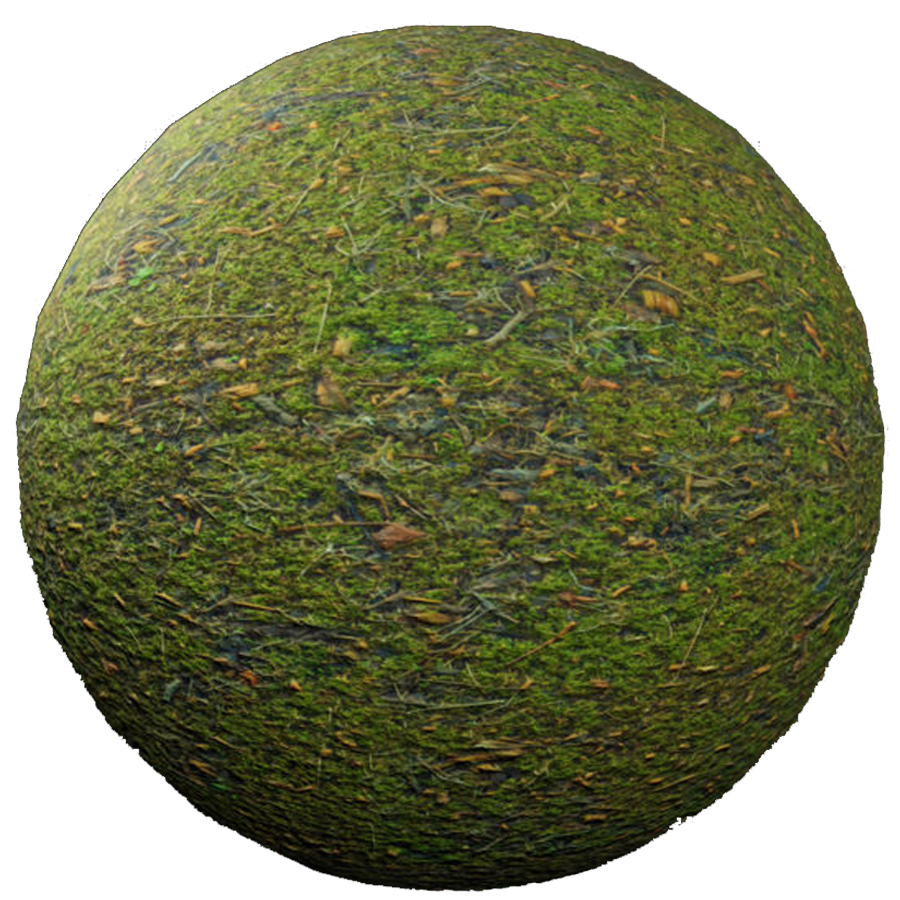
\includegraphics[width=0.24\textwidth]{Memoria/images/mixed_moss.png}
    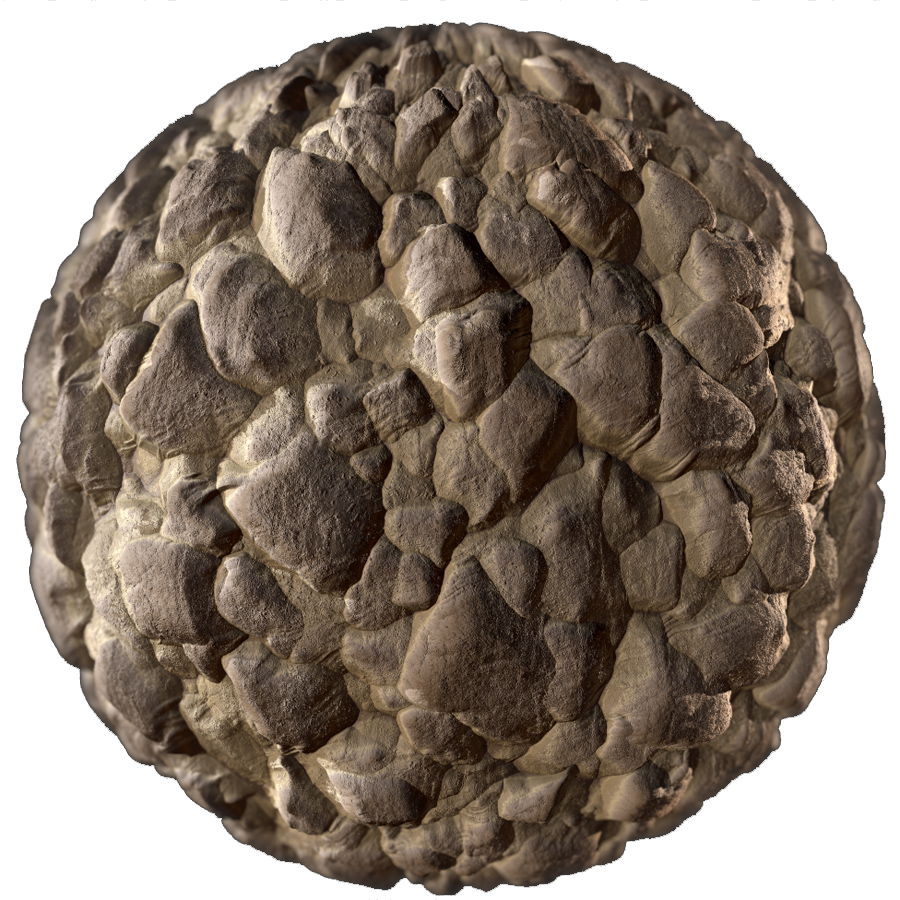
\includegraphics[width=0.24\textwidth]{Memoria/images/badlands_boulder.png}
    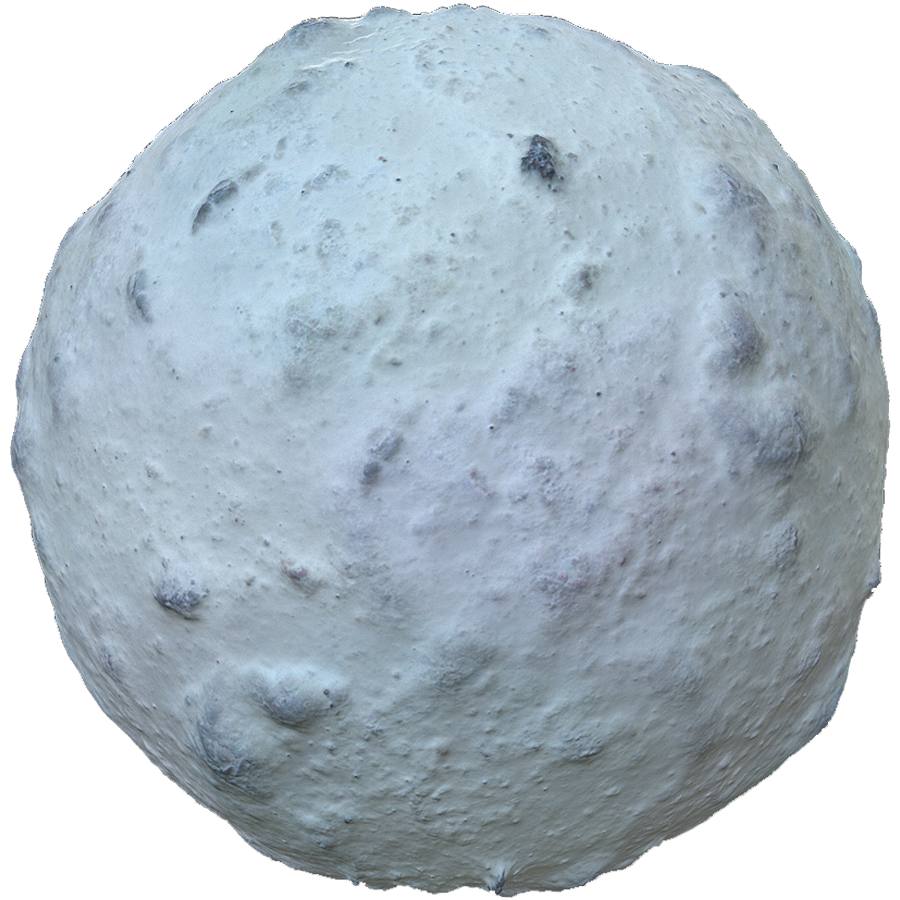
\includegraphics[width=0.24\textwidth]{Memoria/images/rocky_snow.png}
    \caption{Some materials used for terrain.}
    \label{fig:pbr_mats}
\end{figure}
%% ===================================================

\section{Water Shader}
A custom-made shader\footnote{\href{https://github.com/fsande/TFG---Eric-Rios/blob/main/Godot-TerrainGeneration/assets/shaders/water.gdshader}{\textit{Godot-TerrainGeneration/assets/shaders/water.gdshader}}} that emulates water visuals.
Designed to be applied onto a plane mesh representing the sea  as displayed in Figure \ref{fig:sea_plane}.
Blends two normal maps along different directions to emulate waves and modifies the underlying mesh.
Can take a noise texture to imitate foam when close to other geometry.
%Used on sea and rivers.
%% ===================================================
\begin{figure}[H]
    \centering
    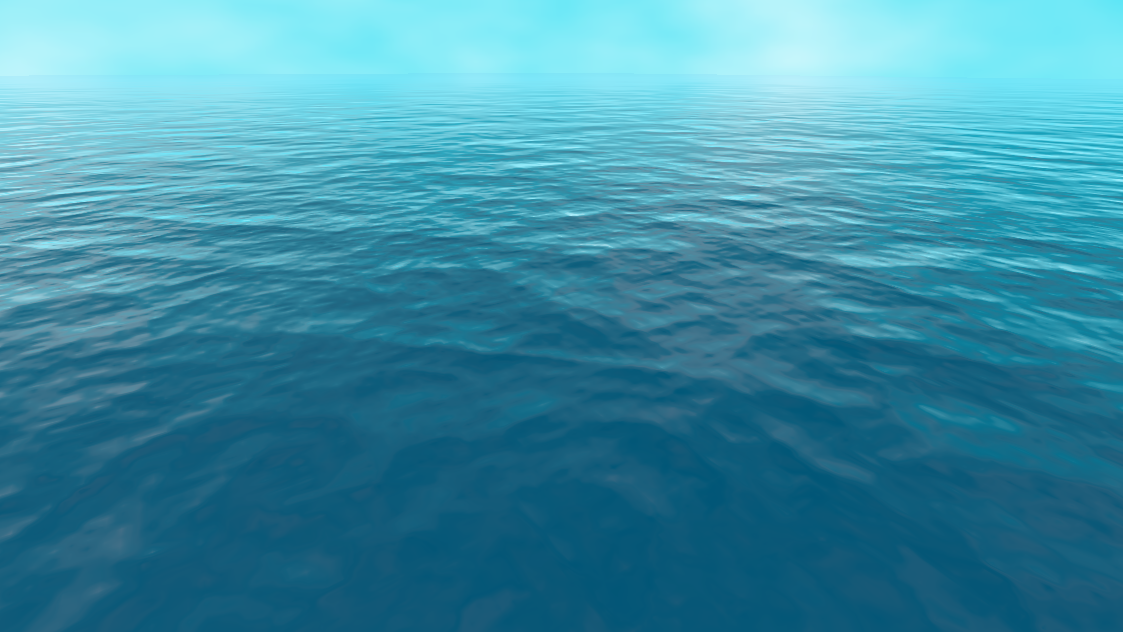
\includegraphics[width=0.6\textwidth]{Memoria/images/sea.png}
    \caption{Plane with water material.}
    \label{fig:sea_plane}
\end{figure}
%% ===================================================

\section{Props}
Trees, bushes and flowers (see Figure \ref{fig:props}) have been sourced from the open source procedural tree generator EZ Tree\footnote{\href{https://www.eztree.dev/}{EZ Tree}. - \url{https://www.eztree.dev/}}.
%% ===================================================
\begin{figure}[H]
    \centering
    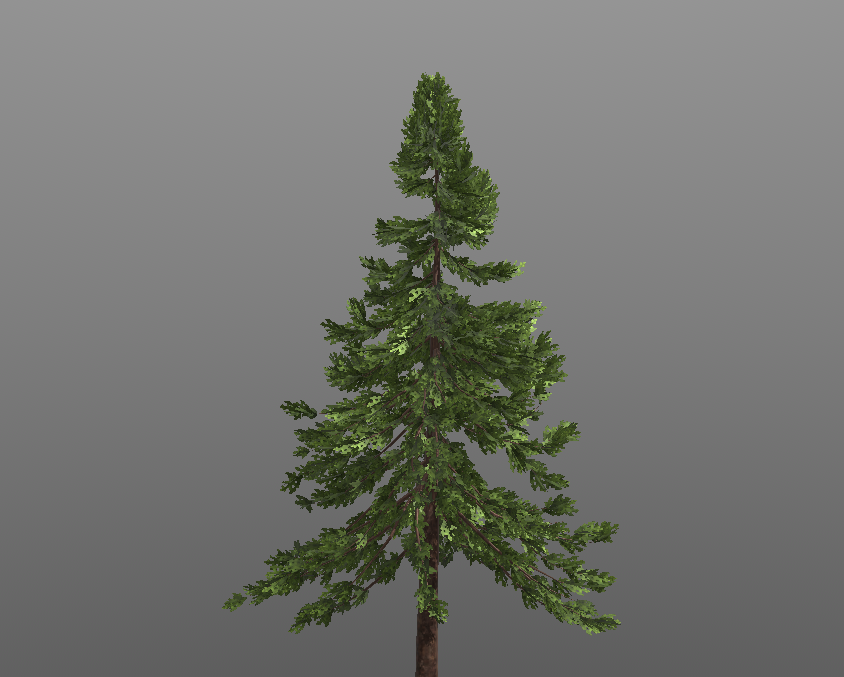
\includegraphics[width=0.32\textwidth]{Memoria/images/tree.png}
    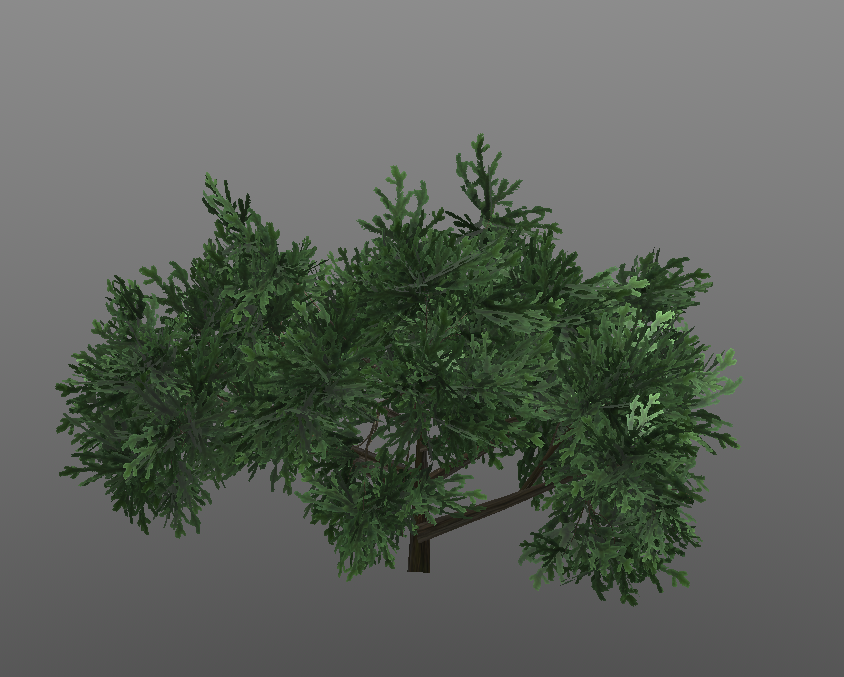
\includegraphics[width=0.32\textwidth]{Memoria/images/bush.png}
    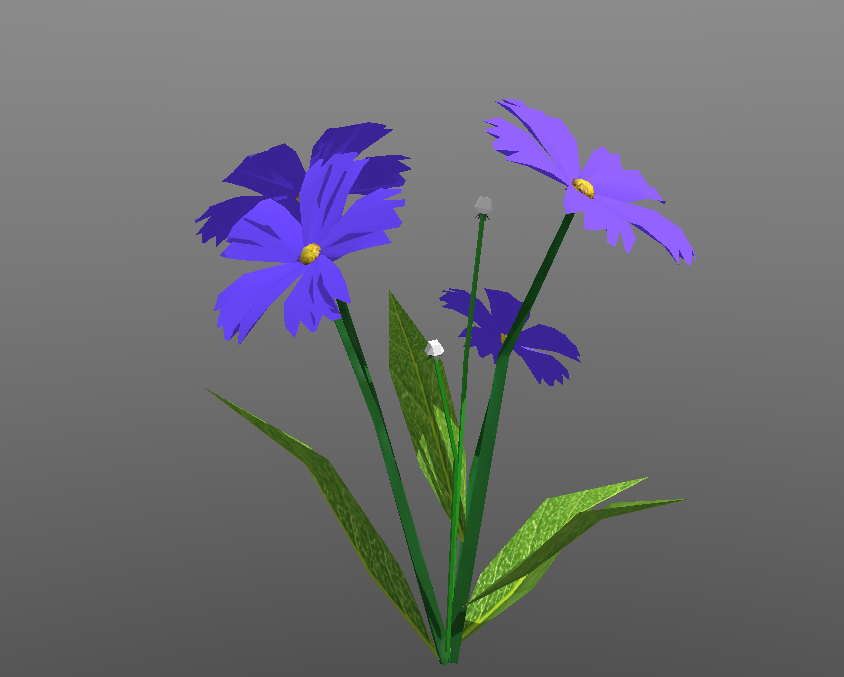
\includegraphics[width=0.32\textwidth]{Memoria/images/flower.png}
    \caption{Some used props.}
    \label{fig:props}
\end{figure}
%% ===================================================

\section{Terrain Shader}
A custom-made shader\footnote{\href{https://github.com/fsande/TFG---Eric-Rios/blob/main/Godot-TerrainGeneration/assets/shaders/advanced_terrain_shader.gdshader}{\textit{Godot-TerrainGeneration/assets/shaders/advanced\_terrain\_shader.gdshader}}} that seamlessly blends different materials at user-defined heights. 
Can take a noise texture to have less uniform blending.
Wrapped by \href{{https://github.com/fsande/TFG---Eric-Rios/blob/main/Godot-TerrainGeneration/materials/height_variation_material.gd}}{\texttt{HeightVariationMaterial}}\footnote{\href{{https://github.com/fsande/TFG---Eric-Rios/blob/main/Godot-TerrainGeneration/materials/height_variation_material.gd}}{\textit{Godot-TerrainGeneration/materials/height\_variation\_material.gd}}} for ease of use and better resource allocation. 
The visual result and the user interface can be seen in Figure \ref{fig:terrain_material}.
\vspace{-0.5em}
%% ===================================================
\begin{figure}[H]
    \centering
    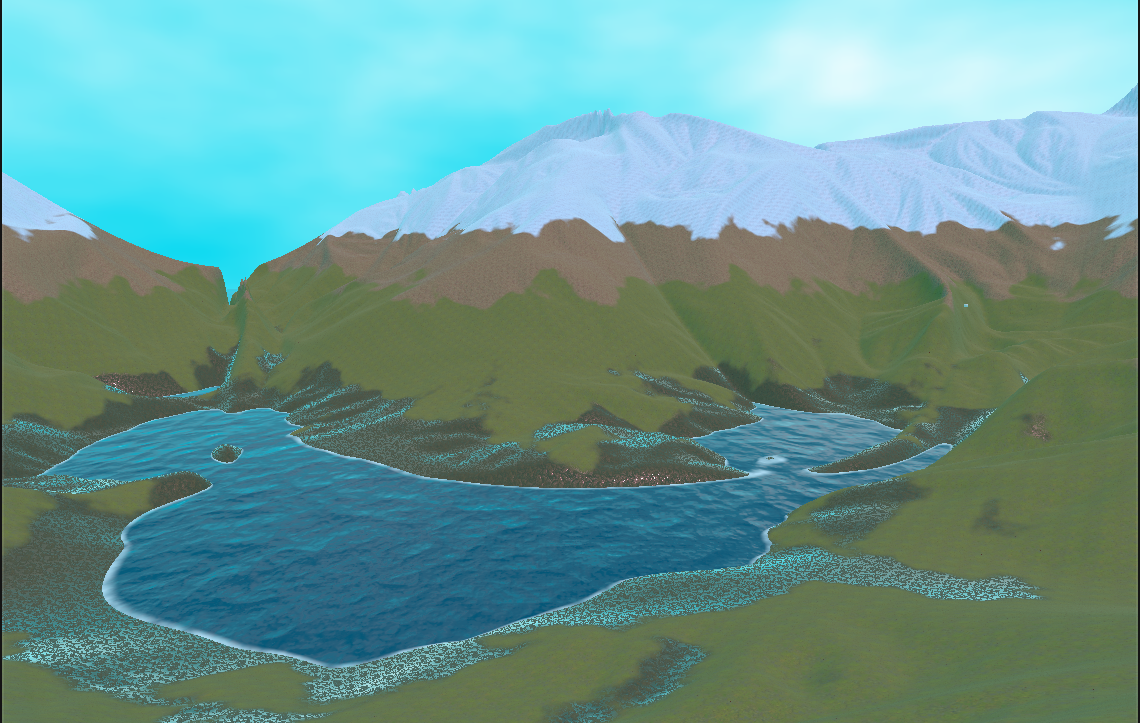
\includegraphics[width=0.65\textwidth]{Memoria/images/terrain_mat_showcase.png}\hfill
    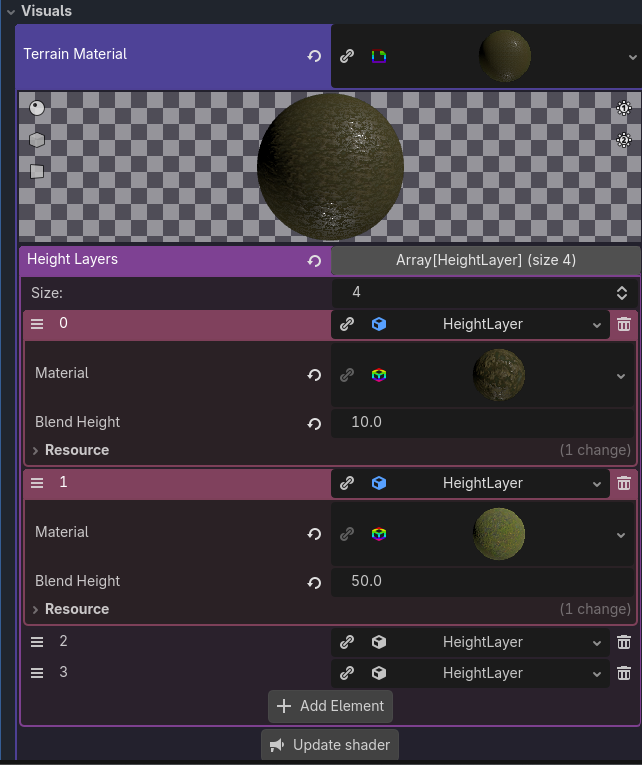
\includegraphics[width=0.35\textwidth]{Memoria/images/terrain_mat_ui.png}
    \caption{Terrain with the material applied and user interface provided by \texttt{\href{https://github.com/fsande/TFG---Eric-Rios/blob/main/Godot-TerrainGeneration/materials/height_variation_material.gd}{\texttt{HeightVariationMaterial}}}.}
    \label{fig:terrain_material}
\end{figure}
%% ===================================================